\documentclass[11pt]{article}

\usepackage[utf8]{inputenc}
\usepackage[portuges]{babel}
\usepackage{indentfirst}
\usepackage{natbib}
\usepackage{graphicx}

\renewcommand{\contentsname}{Índice}

\begin{document}

\begin{titlepage}
    \begin{center}
        
\includegraphics[width=0.3\textwidth]{images/capa/EscolaEngenhariaUM.jpeg}
    
        \vspace{1cm}
        
        \textbf{\LARGE Redes de Computadores}
    
        \vspace{0.5cm}
        \textbf{\Large Trabalho Prático 2}

        \vspace{1.3cm}
        
        \textbf{\large Francisco Correia Franco A89458 \\
        António Jorge Nande Rodrigues A89585 \\
        Luís Enes Sousa A89597}

        \vspace{1.5cm}
    
        \begin{figure}[hbt!]
        \minipage{0.32\textwidth}
            
\includegraphics[width=\linewidth]{images/capa/152.png}
            \centering
            \captionsetup{A89458}
        \endminipage\hfill
        \minipage{0.32\textwidth}
            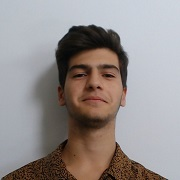
\includegraphics[width=\linewidth]{images/capa/133.jpeg}
            \centering
            \captionsetup{A89585}
        \endminipage\hfill
        \minipage{0.32\textwidth}
            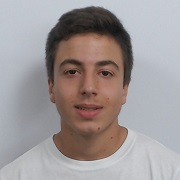
\includegraphics[width=\linewidth]{images/capa/80.jpeg}
            \centering
            \captionsetup{A89597}
        \endminipage
        \end{figure}
    \end{center}
\end{titlepage}

\tableofcontents
\thispagestyle{empty}
\cleardoublepage

\setcounter{page}{1}


%------------------------------------------------------------------------------------------------------%


\section{Captura de tráfego IP}

\vspace{0.5cm}

\subsection{Pergunta 1}

Prepare uma topologia CORE para verificar o comportamento do
traceroute. Ligue um host (pc) Cliente1 a um router R2; o router
R2 a um router R3, que por sua vez, se liga a um host (servidor)
Servidor1. (Note que pode não existir conectividade IP imediata
entre o Cliente1 e o Servidor1 até que o anúncio de rotas
estabilize).

\begin{figure}[hbt!]
    \centering
    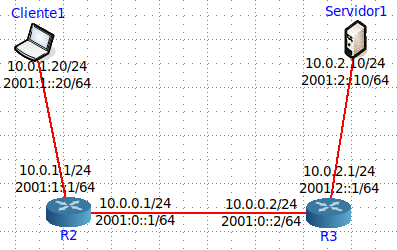
\includegraphics[width=0.7\textwidth]{images/parte1/topologia/core.png}
    \caption{Topologia CORE}
\end{figure}

\vspace{0.5cm}

\textbf{A - Ative o wireshark ou o tcpdump no pc h1. Numa shell de h1, execute o comando traceroute -I para o endereço IP do host s4.}

\begin{figure}[hbt!]
    \centering
    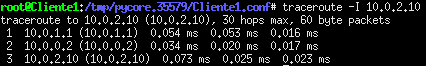
\includegraphics[width=1\textwidth]{images/parte1/topologia/t_route.png}
    \caption{Traceroute do Cliente1 para o Servidor1}
\end{figure}

\clearpage

\textbf{B - Registe e analise o tráfego ICMP enviado pelo Cliente1 e o tráfego ICMP recebido como resposta. Comente os resultados face ao comportamento esperado.}

Inicialmente, o Cliente1 tenta comunicar com o Servidor1, mas, como o TTL é igual a 1, o pacote vai ser descartado ao chegar a R2, sendo retribuída uma mensagem de erro ao Cliente1. O TTL é, então, aumentado sucessivamente, até chegar a TTL 3, que é o mínimo necessário para chegar ao Servidor1.

\begin{figure}[hbt!]
    \centering
    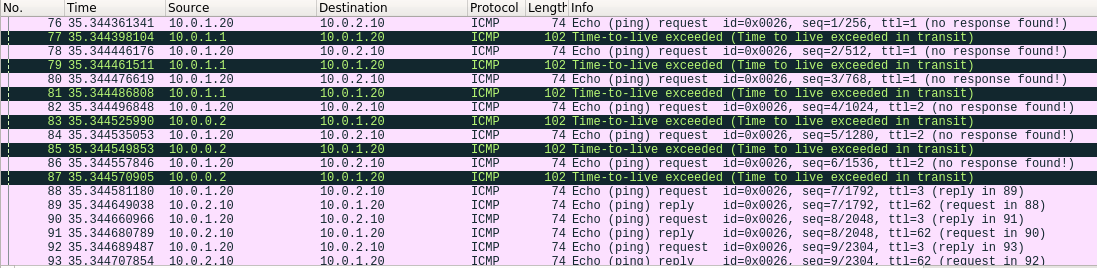
\includegraphics[width=\textwidth]{images/parte1/topologia/trafego_icmp.png}
    \caption{Tráfego ICMP}
\end{figure}

\vspace{0.5cm}

\textbf{C - Qual deve ser o valor inicial mínimo do campo TTL para alcançar o Servidor1? Verifique na prática que a sua resposta está correta.}

O valor inicial do campo TTL deverá ser 3. Na figura 3 podemos verificar que o valor mais baixo do TTL para o qual o pacote chega ao destino é 3.

\vspace{1cm}

\textbf{D - Calcule o valor médio do tempo de ida-e-volta (Round-Trip Time) obtido?}

O Round-Trip Time médio deverá ser 0.020 ms.

\begin{figure}[hbt!]
    \centering
    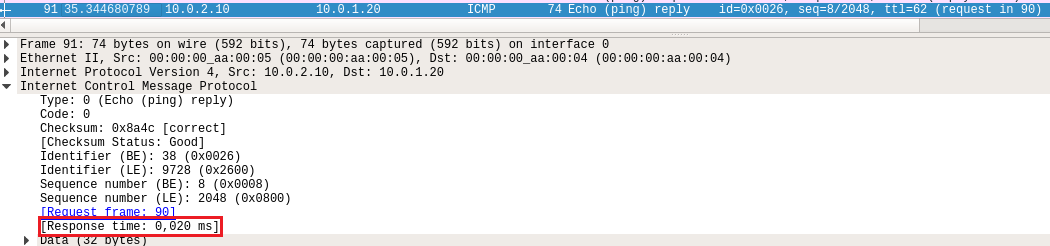
\includegraphics[width=\textwidth]{images/parte1/topologia/round_trip.png}
    \caption{Round-Trip Time}
\end{figure}

\subsection{Pergunta 2}

Pretende-se agora usar o traceroute na sua máquina nativa, e gerar de datagramas IP de diferentes tamanhos.

Selecione a primeira mensagem ICMP capturada e centre a análise no nível protocolar IP. Através da análise do cabeçalho IP diga: 

\vspace{0.5cm}

\textbf{A - Qual é o endereço IP da interface ativa do seu computador?}

O endereço IP da interface ativa do nosso computador é 172.26.9.103.

\begin{figure}[hbt!]
    \centering
    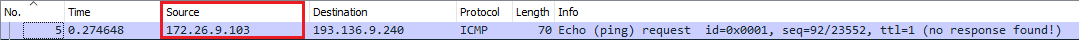
\includegraphics[width=\textwidth]{images/parte1/default/endereco_ip.png}
    \caption{Endereço IP da interface ativa}
\end{figure}

\vspace{0.5cm}

\textbf{B - Qual é o valor do campo protocolo? O que identifica?}

O campo protocolo é igual a 1, referente ao protocolo ICMP (Internet Control Message Protocol).

\begin{figure}[hbt!]
    \centering
    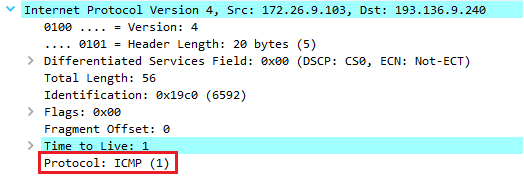
\includegraphics[width=\textwidth]{images/parte1/default/campo_protocolo.png}
    \caption{Valor do campo protocolo}
\end{figure}

\clearpage

\textbf{C - Quantos bytes tem o cabeçalho IP(v4)? Quantos bytes tem o campo de dados (payload) do datagrama? Como se calcula o tamanho do payload?}

O cabeçalho IP(v4) tem 20 bytes.

O campo de dados tem um tamanho de 36 bytes. Este valor é calculado através da diferença do tamanho total (56 bytes) com o tamanho do cabeçalho (20 bytes).

\begin{figure}[hbt!]
    \centering
    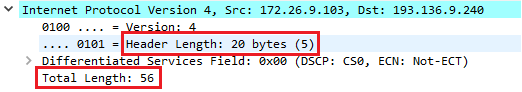
\includegraphics[width=\textwidth]{images/parte1/default/header_total_length.png}
    \caption{Header e Total Length}
\end{figure}

\vspace{0.5cm}

\textbf{D - O datagrama IP foi fragmentado? Justifique.}

O valor das flags e do offset é igual a 0, logo o pacote não foi fragmentado.

\begin{figure}[hbt!]
    \centering
    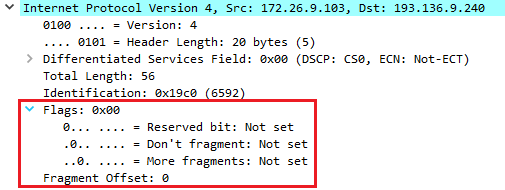
\includegraphics[width=\textwidth]{images/parte1/default/flags.png}
    \caption{Flags e Offset}
\end{figure}

\clearpage

\textbf{E -  Ordene os pacotes capturados de acordo com o endereço IP fonte (e.g., selecionando o cabeçalho da coluna Source), e analise a sequência de tráfego ICMP gerado a partir do endereço IP atribuído à interface da sua máquina. Para a sequência de mensagens ICMP enviadas pelo seu computador, indique que campos do cabeçalho IP variam de pacote para pacote.}

Os campos do cabeçalho IP que variam são o campo de identificação e o TTL.

\begin{figure}[hbt!]
    \minipage{0.49\textwidth}
        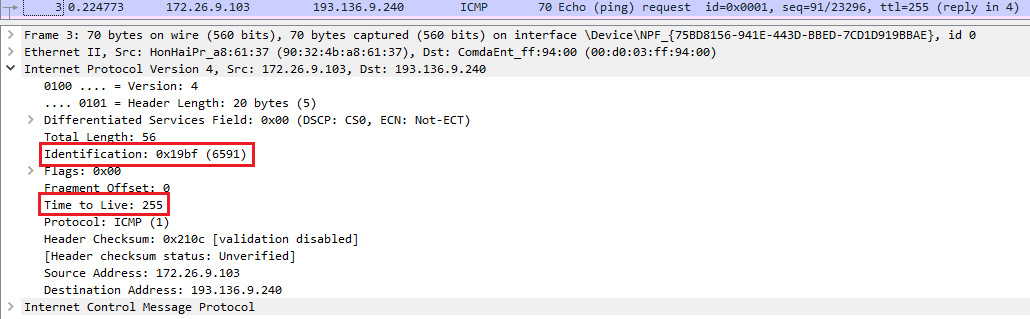
\includegraphics[width=\linewidth]{images/parte1/default/pacote1.png}
        \centering
        \captionsetup{Pacote 1}
    \endminipage\hfill
    \minipage{0.49\textwidth}
        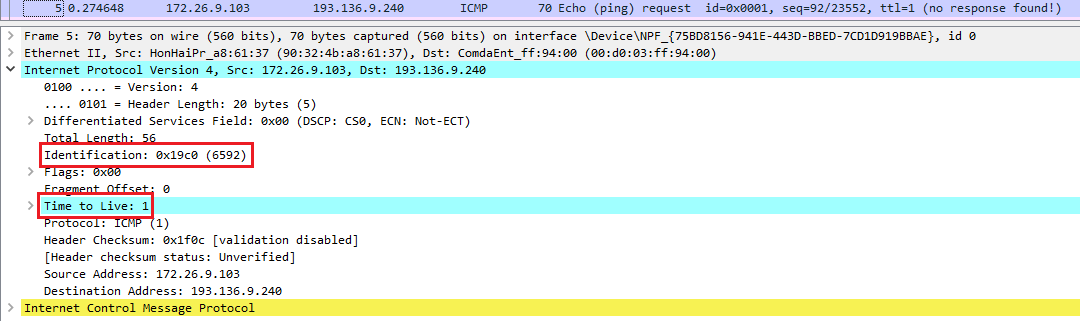
\includegraphics[width=\linewidth]{images/parte1/default/pacote2.png}
        \centering
        \captionsetup{Pacote 2}
    \endminipage
    \caption{Exemplo de dois pacotes enviados pelo computador}
\end{figure}

\vspace{0.5cm}

\textbf{F - Observa algum padrão nos valores do campo de Identificação do datagrama IP e TTL?}

Como se pode ver na Figura 9, referente a dois pacotes consecutivos, o campo de identificação é incrementado a cada pacote enviado.

Na Figura 10 verifica-se que o TTL também é incrementado a cada pacote enviado. No entanto, a cada 5 pacotes é enviado um pacote de teste (TTL = 255).

\begin{figure}[hbt!]
    \centering
    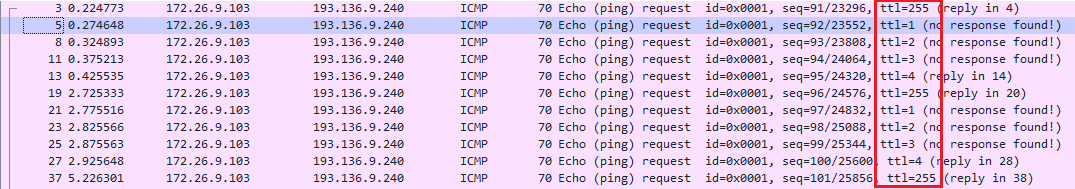
\includegraphics[width=\textwidth]{images/parte1/default/ttl_evolving.png}
    \caption{Evolução do TTL}
\end{figure}

\clearpage

\textbf{G - Ordene o tráfego capturado por endereço destino e encontre a série de respostas ICMP TTL exceeded enviadas ao seu computador. Qual é o valor do campo TTL? Esse valor permanece constante para todas as mensagens de resposta ICMP TTL exceeded enviados ao seu host? Porquê?}

A Figura 12 mostra os diferentes valores dos TTL. O primeiro pacote tem TTL=255, o segundo TTL=254 e o terceiro TTL=253. Isto deve-se ao facto dos TTL enviados pelo nosso router serem incrementados ao longo do tempo fazendo com que cheguem mais longe e saltem por mais routers. Quando é necessário enviar uma mensagem de erro os pacotes são enviados do router mais distante até ao nosso router. Sendo assim, quanto maior o TTL do pacote enviado, menor o TTL do pacote recebido (vindo do router que enviou a mensagem de erro), pois este último tem de passar por mais routers intermédios, tendo o seu TTL sido decrementado em cada um.

\begin{figure}[hbt!]
    \centering
    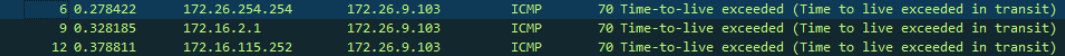
\includegraphics[width=\textwidth]{images/parte1/default/pacotes_destination.png}
    \caption{Pacotes ordenados por destino}
\end{figure}

\begin{figure}[hbt!]
    \minipage{0.32\textwidth}
        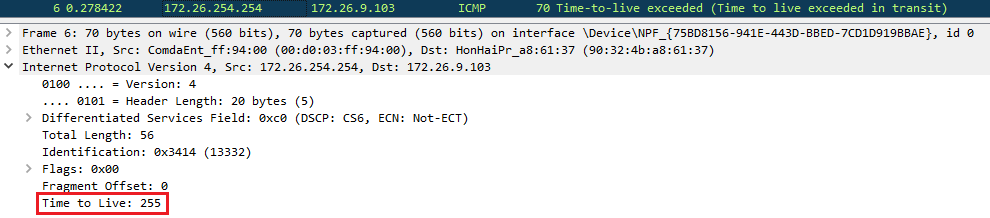
\includegraphics[width=\linewidth]{images/parte1/default/ttl_255.png}
        \centering
        \captionsetup{1º Pacote}
    \endminipage\hfill
    \minipage{0.32\textwidth}
        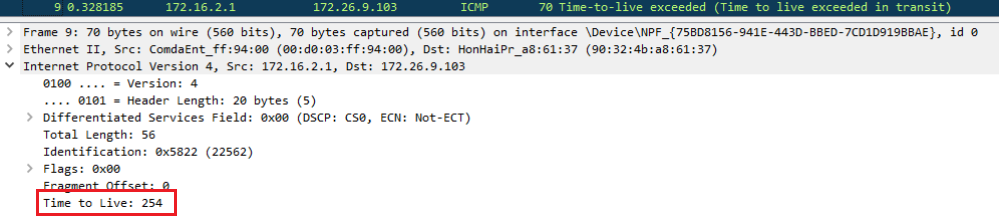
\includegraphics[width=\linewidth]{images/parte1/default/ttl_254.png}
        \centering
        \captionsetup{2º Pacote}
    \endminipage\hfill
    \minipage{0.32\textwidth}
        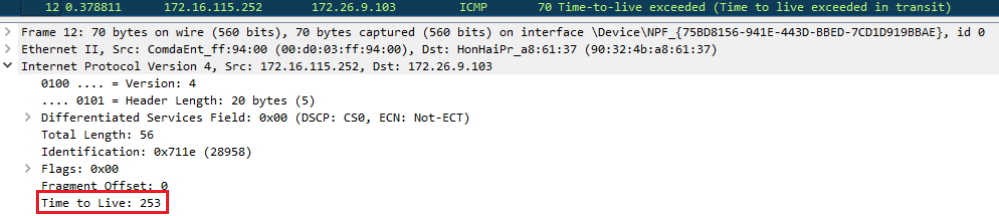
\includegraphics[width=\linewidth]{images/parte1/default/ttl_253.png}
        \centering
        \captionsetup{3º Pacote}
    \endminipage
    \caption{Exemplo de três pacotes consecutivos recebidos pelo computador}
\end{figure}

\clearpage
\subsection{Pergunta 3}

Pretende-se agora analisar a fragmentação de pacotes IP.

Observe o tráfego depois do tamanho de pacote ter sido  definido para 32XX bytes.

\vspace{0.5cm}

\textbf{A - Localize a primeira mensagem ICMP. Porque é que houve necessidade de fragmentar o pacote inicial? }

O pacote inicial teve de ser fragmentado, pois este tem 3252 bytes e o MTU (Maximum Transport Unit) da rede é 1500 bytes. Assim, o pacote tem de ser fragmentado em três partes, para poder seguir nesta rede.

\begin{figure}[hbt!]
    \centering
    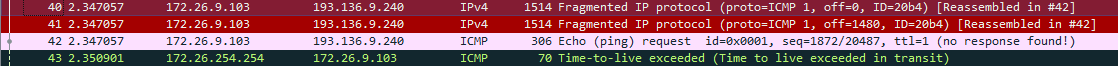
\includegraphics[width=\textwidth]{images/parte1/3252/primeiro_icmp.png}
    \caption{Primeira mensagem ICMP}
\end{figure}

\vspace{0.5cm}

\textbf{B - Imprima o primeiro fragmento do datagrama IP segmentado. Que informação no cabeçalho indica que o datagrama foi fragmentado? Que informação no cabeçalho IP indica que se trata do primeiro fragmento? Qual é o tamanho deste datagrama IP?}

Pode-se concluir que o datagrama foi fragmentado, pois as flags têm um valor diferente de 0.

O facto de 'Fragment Offset' ser 0 e a flag 'More fragments' ser 1 indica que se trata do primeiro fragmento.

O tamanho deste datagrama IP é 1500 bytes.

\begin{figure}[hbt!]
    \centering
    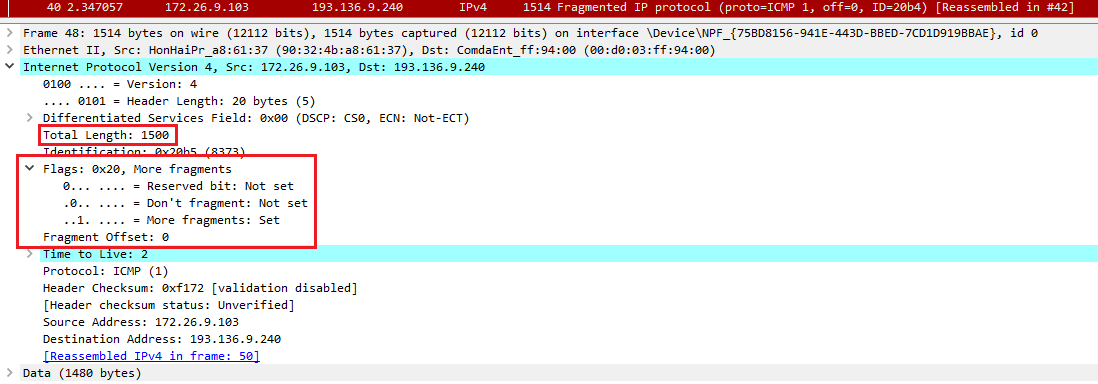
\includegraphics[width=\textwidth]{images/parte1/3252/primeiro_fragmento.png}
    \caption{Primeiro fragmento do datagrama IP segmentado}
\end{figure}

\clearpage

\textbf{C - Imprima o segundo fragmento do datagrama IP original. Que informação do cabeçalho IP indica que não se trata do 1º fragmento? Há mais fragmentos? O que nos permite afirmar isso?}

O 'Fragment Offset' é igual a 1480 (diferente de 0), logo não se trata do primeiro fragmento.

Como o datagrama tem a flag 'More Fragments' a 1, pode-se concluir que há mais fragmentos.

\begin{figure}[hbt!]
    \centering
    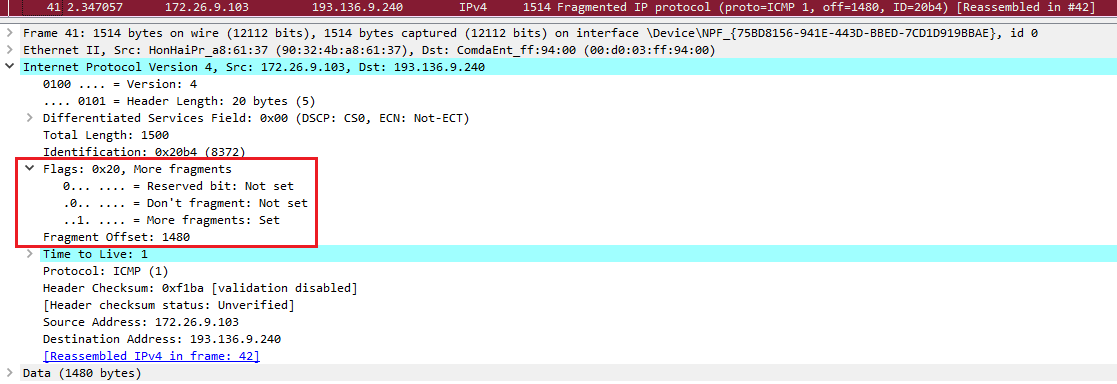
\includegraphics[width=\textwidth]{images/parte1/3252/segundo_fragmento.png}
    \caption{Segundo fragmento do datagrama IP segmentado}
\end{figure}

\vspace{0.4cm}

\textbf{D - Quantos fragmentos foram criados a partir do datagrama original? Como se detecta o último fragmento correspondente ao datagrama original?}

Foram criados 3 fragmentos a partir do datagrama original.

Sabe-se que este é o último fragmento do datagrama original, pois a flag 'More Fragments' está a 0 e o 'Fragment Offset' é diferente de 0.

\begin{figure}[hbt!]
    \centering
    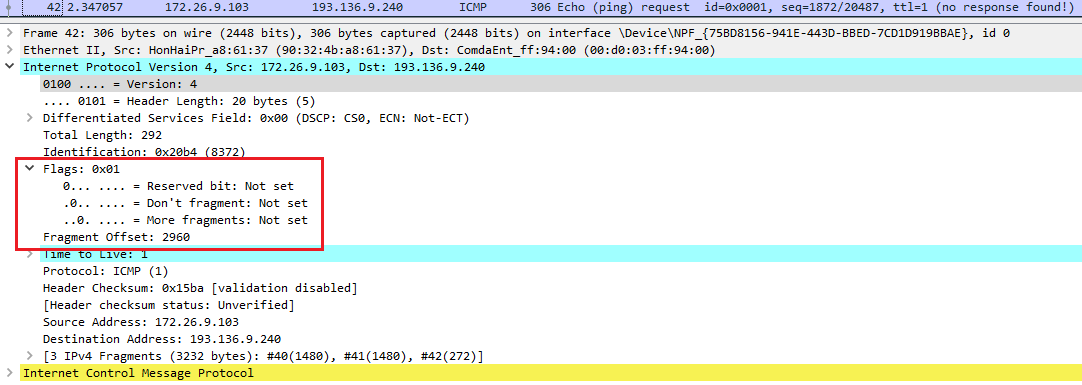
\includegraphics[width=\textwidth]{images/parte1/3252/ultimo_fragmento.png}
    \caption{Último fragmento do datagrama IP segmentado}
\end{figure}


\textbf{E - Indique, resumindo, os campos que mudam no cabeçalho IP entre os diferentes fragmentos, e explique a forma como essa informação permite reconstruir o datagrama original.}

Os campos que mudam entre os diferentes fragmentos são as flags 'More Fragments' e 'Fragment Offset'.

A flag 'More Fragments' indica se existem mais fragmentos. Já a flag 'Fragment Offset' permite identificar a posição do fragmento no datagrama original. Assim, é possível reconstruir o datagrama original juntando os fragmentos por ordem crescente do valor da flag 'Fragment Offset'.


%------------------------------------------------------------------------------------------------------%


\clearpage
\section{Endereçamento e Encaminhamento IP}

Considere que a organização MIEI-RC é constituída por quatro
departamentos (A, B, C e D) e cada departamento possui um router de
acesso à sua rede local. Estes routers de acesso (RA, RB, RC e RD) estão interligados entre si por ligações Ethernet a 1Gbps, formando um anel.

Por sua vez, existe um servidor (S1) na rede do departamento A e, pelo menos, dois laptops por departamento, interligados ao router respetivo através de um comutador (switch). S1 tem uma ligação a 1Gbps e os laptops ligações a 100Mbps. Considere apenas a existência de um comutador por departamento.

A conectividade IP externa da organização é assegurada através de um router de acesso RISP conectado a RA por uma ligação ponto-a-ponto a 10 Gbps.

\vspace{0.5cm}

\subsection{Pergunta 1}

\textbf{A - Indique que endereços IP e máscaras de rede foram
atribuídos pelo CORE a cada equipamento. Para simplificar,
pode incluir uma imagem que ilustre de forma clara a
topologia definida e o endereçamento usado.}

A imagem seguinte ilustra os vários endereços IP e a respetiva máscara (255.255.255.0, ou /24 em notação CIDR) atribuídos pelo CORE a cada equipamento.

\begin{figure}[!htb]
    \centering
    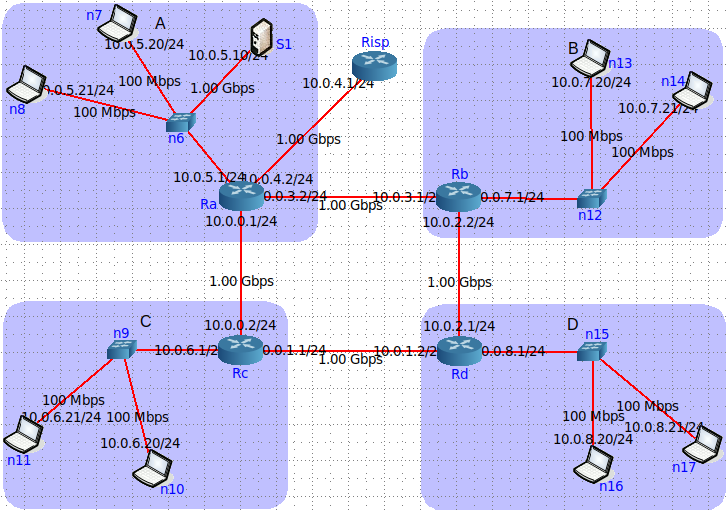
\includegraphics[width=0.5\textwidth]{images/parte2/core.png}
    \caption{Topologia CORE}
\end{figure}

\clearpage
\textbf{B - Tratam-se de endereços públicos ou privados? Porquê?}

Tratam-se de endereços privados, pois pertencem à Classe A (endereços entre 10.0.0.0 e 10.255.255.255).

\vspace{0.5cm}

\textbf{C - Porque razão não é atribuído um endereço IP aos switches?}

O switch tem como principal função a interligação de equipamentos. Na primeira vez que um pacote é reencaminhado para um equipamento, o switch guarda o endereço MAC na sua tabela de endereços MAC (onde são guardados os endereços MAC dos equipamentos ligados a cada porta do switch).

Através da informação contida na sua tabela de endereços MAC, o switch é capaz de fazer o redirecionamento de pacotes entre os equipamentos ligados a ele.

\vspace{0.5cm}

\textbf{D - Usando o comando ping certifique-se que existe conectividade IP entre os laptops dos vários departamentos e o servidor do departamento A (basta certificar-se da conectividade de um laptop por departamento).}

Como podemos ver pelas imagens seguintes, os equipamentos de cada departamento conseguem receber e enviar pacotes entre eles e o servidor do departamento C. Sendo assim, conclui-se que existe conectividade IP entre os mesmos.

\begin{figure}[hbt!]
    \minipage{0.45\textwidth}
        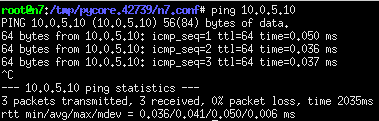
\includegraphics[width=\linewidth]{images/parte2/depA.png}
        \centering
        \captionsetup{Departamento A}
    \endminipage\hfill
    \minipage{0.45\textwidth}
        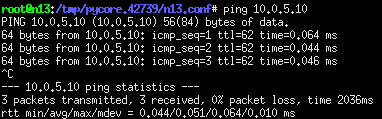
\includegraphics[width=\linewidth]{images/parte2/depB.png}
        \centering
        \captionsetup{Departamento B}
    \endminipage
    \vspace{0.2cm}
    \minipage{0.45\textwidth}
        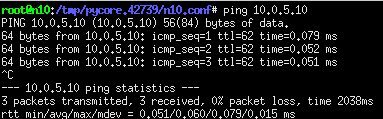
\includegraphics[width=\linewidth]{images/parte2/depC.png}
        \centering
        \captionsetup{Departamento C}
    \endminipage\hfill
    \minipage{0.45\textwidth}
        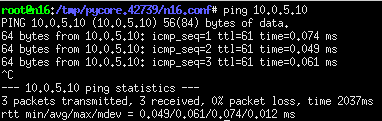
\includegraphics[width=\linewidth]{images/parte2/depD.png}
        \centering
        \captionsetup{Departamento D}
    \endminipage
    \caption{Ping dos departamentos para o servidor S1}
\end{figure}

\clearpage

\textbf{E - Verifique se existe conectividade IP do router de acesso RISP para o servidor S1.}

Usando o mesmo método da pergunta anterior, verifica-se que existe conectividade IP entre o router RISP e o servidor S1.

\begin{figure}[!htb]
    \centering
    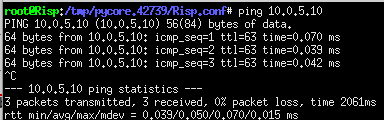
\includegraphics[width=0.5\textwidth]{images/parte2/Risp.png}
    \caption{Ping do Router RISP para o servidor S1}
\end{figure}

\vspace{0.5cm}

\subsection{Pergunta 2}

Para o router e um laptop do departamento C:

\vspace{0.5cm}

\textbf{A - Execute o comando netstat –rn por forma a poder consultar a tabela de encaminhamento unicast (IPv4). Inclua no seu relatório as tabelas de encaminhamento obtidas; interprete as várias entradas de cada tabela. Se necessário, consulte o manual respetivo (man netstat).}

A tabela de encaminhamento do laptop tem duas entradas. A linha da coluna 'Destination' com valor 0.0.0.0 (default) informa que um pacote que pretenda ser enviado para uma rede desconhecida deve seguir pelo respetivo Gateway. A outra linha, com o valor 10.0.6.0, é usada quando se pretende enviar um pacote para a própria rede.

\begin{figure}[!htb]
    \centering
    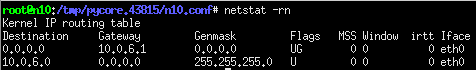
\includegraphics[width=0.5\textwidth]{images/parte2/laptopC.png}
    \caption{Tabela de encaminhamento do laptop}
\end{figure}

\clearpage
A tabela de encaminhamento do router contém as redes alcançáveis pelo router e os respetivos gateways.
Quando o destino de um pacote corresponde a um dos valores da coluna 'Destination', o pacote é enviado pelo respetivo valor na coluna 'Gateway'.

\begin{figure}[!htb]
    \centering
    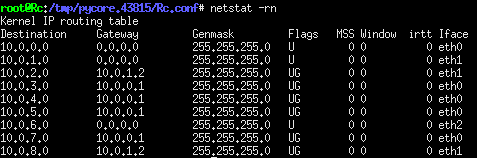
\includegraphics[width=0.5\textwidth]{images/parte2/routerC.png}
    \caption{Tabela de encaminhamento do router}
\end{figure}

\vspace{0.5cm}

\textbf{B - Diga, justificando, se está a ser usado encaminhamento estático ou dinâmico (sugestão: analise que processos estão a correr em cada sistema, por exemplo, ps -ax).}

No router, está a ser usado encaminhamento dinâmico, pois o comando “ps -ax” mostra que estão a correr processos com o protocolo OSPF e ZEBRA. No encaminhamento dinâmico os routers trocam informação de routing entre si, sendo as rotas atualizadas ao longo do tempo.

\begin{figure}[!htb]
    \centering
    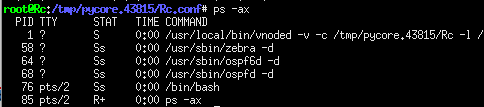
\includegraphics[width=0.5\textwidth]{images/parte2/ps_routerC.png}
    \caption{Processos a correr no router}
\end{figure}

Pelo contrário, no laptop o encaminhamento é estático, pois apenas estão a correr os processos básicos da máquina. No encaminhamento estático as rotas permanecem fixas e são baseadas nas rotas pré-definidas.

\begin{figure}[!htb]
    \centering
    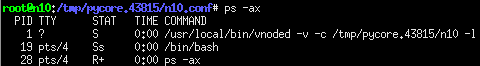
\includegraphics[width=0.5\textwidth]{images/parte2/ps_laptopC.png}
    \caption{Processos a correr no laptop}
\end{figure}

\clearpage
\textbf{C - Admita que, por questões administrativas, a rota por defeito (0.0.0.0 ou default) deve ser retirada definitivamente da tabela de encaminhamento do servidor S1 localizado no departamento A. Use o comando route delete para o efeito.
Que implicações tem esta medida para os utilizadores da organização MIEI-RC que acedem ao servidor. Justifique.}

Ao retirar a rota por defeito, o servidor S1 deixa de conseguir comunicar com equipamentos fora da sua rede (10.0.5.0). Isto acontece pois a tabela de encaminhamento do servidor passa a conter apenas informação de como enviar pacotes para a rede 10.0.5.0. Todos os pacotes com destino diferente são descartados, pois o servidor não sabe para onde os enviar. 

\begin{figure}[!htb]
    \centering
    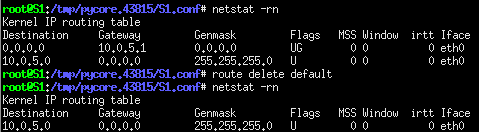
\includegraphics[width=0.5\textwidth]{images/parte2/serv1.png}
    \caption{Tabela de encaminhamento do servidor S1}
\end{figure}

\vspace{0.5cm}

\textbf{D - Adicione as rotas estáticas necessárias para restaurar a conectividade para o servidor S1, por forma a contornar a restrição imposta na alínea c). Utilize para o efeito o comando route add e registe os comandos que usou.}

\begin{figure}[!htb]
    \centering
    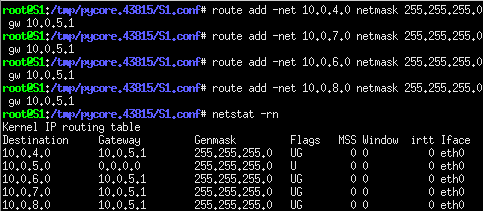
\includegraphics[width=0.5\textwidth]{images/parte2/add_rotas.png}
    \caption{Rotas adicionadas para os departamentos e para o router de acesso}
\end{figure}

\clearpage
\textbf{E - Teste a nova política de encaminhamento garantindo que o servidor está novamente acessível, utilizando para o efeito o comando ping. Registe a nova tabela de encaminhamento do servidor.}

Nas imagens seguintes verifica-se que os diversos equipamentos (Laptops dos departamentos B, C e D e router RISP) conseguem transmitir pacotes com o servidor S1, concluindo-se que este está novamente acessível.

\begin{figure}[hbt!]
    \minipage{0.45\textwidth}
        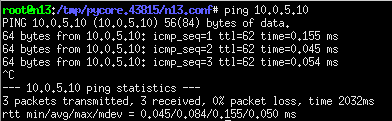
\includegraphics[width=\linewidth]{images/parte2/depB_2.png}
        \centering
        \captionsetup{Departamento B}
    \endminipage\hfill
    \minipage{0.45\textwidth}
        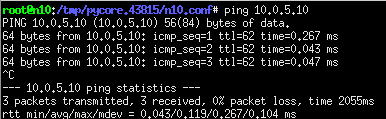
\includegraphics[width=\linewidth]{images/parte2/depC_2.png}
        \centering
        \captionsetup{Departamento C}
    \endminipage
    \vspace{0.2cm}
    \minipage{0.45\textwidth}
        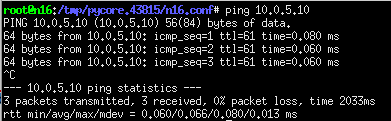
\includegraphics[width=\linewidth]{images/parte2/depD_2.png}
        \centering
        \captionsetup{Departamento D}
    \endminipage\hfill
    \minipage{0.45\textwidth}
        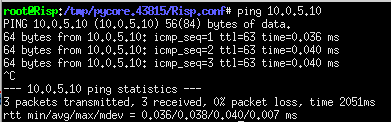
\includegraphics[width=\linewidth]{images/parte2/Risp_2.png}
        \centering
        \captionsetup{Router RISP}
    \endminipage
    \caption{Ping dos departamentos e do router RISP para o servidor S1}
\end{figure}


%------------------------------------------------------------------------------------------------------%


\clearpage
\section{Definição de Sub-redes}

Considere a topologia definida anteriormente. Assuma que o endereçamento entre os routers se mantém inalterado, contudo, o endereçamento em cada departamento deve ser redefinido.

\vspace{1cm}

\subsection{Pergunta 1}

Considere que dispõe apenas do endereço de rede IP 130.XX.96.0/19, em que XX é o decimal correspondendo ao seu número de grupo (PLXX). Defina um novo esquema de endereçamento para as redes dos departamentos (mantendo a rede de acesso e core inalteradas) e atribua endereços às interfaces dos vários sistemas envolvidos. Assuma que todos os endereços de sub-redes são usáveis. Deve justificar as opções usadas.

\vspace{0.5cm}

O nosso endereço de rede é 130.52.96.0/19. Uma vez que temos uma máscara de 19 significa que a nossa rede pode usar todos os endereços entre 130.52.96.0 e 130.52.127.255.

Como temos 4 departamentos, são necessários 2 bits para conseguir atribuir um endereço a cada departamento (sub-netting). No entanto, é boa prática deixar um endereço disponível entre cada sub-rede, caso seja preciso aumentar o número de hosts de um departamento. Desta forma, garante-se que, à medida que os IPs aumentam, a ordem alfabética dos departamentos também.

Usando 3 bits, temos então 8 opções disponíveis para fazer sub-netting. Assim, distribuímos os endereços seguindo o modelo \textbf{130.52.011XXX00.0}, em que XXX são os bits atribuídos a cada departamento.

\begin{table}[hbt!]
    \centering
    \begin{tabular}{|l|l|}
    \hline
    \multicolumn{1}{|c|}{000} & Dep A \\ \hline
    001                       & Livre (Dep A) \\ \hline
    010                       & Dep B \\ \hline
    011                       & Livre (Dep B) \\ \hline
    100                       & Dep C \\ \hline
    101                       & Livre (Dep C) \\ \hline
    110                       & Dep D \\ \hline
    111                       & Livre (Dep D) \\ \hline
    \end{tabular}
    \caption{Bits atribuídos a cada departamento}
\end{table}

\begin{table}[htb!]
    \centering
    \begin{tabular}{|c|c|c|c|}
    \hline
    Dep. & IP              & IP inicial   & IP final       \\ \hline
    A    & 130.52.96.0/22  & 130.52.96.0  & 130.52.99.255  \\ \hline
    B    & 130.52.104.0/22 & 130.52.104.0 & 130.52.107.255 \\ \hline
    C    & 130.52.112.0/22 & 130.52.112.0 & 130.52.115.255 \\ \hline
    D    & 130.52.120.0/22 & 130.52.120.0 & 130.52.123.255 \\ \hline
    \end{tabular}
    \caption{IPs de host para cada departamento}
\end{table}

Assim, conseguimos atribuir um IP a cada equipamento, dentro do intervalo disponibilizado para cada departamento (exceto os IPs com tudo a 0 e tudo a 1).

\begin{table}[htb!]
    \centering
    \begin{tabular}{|c|c|c|c|}
    \hline
    \textbf{Dep A} & \textbf{IP atribuído} & \textbf{Dep B} & \textbf{IP atribuído} \\ \hline
    n7             & 130.52.96.2/22        & n13            & 130.52.104.2/22       \\ \hline
    n8             & 130.52.96.3/22        & n14            & 130.52.104.3/22       \\ \hline
    S1             & 130.52.96.4/22        & Rb             & 130.52.104.1/22       \\ \hline
    Ra             & 130.52.96.1/22        & -              & -                     \\ \hline
    \textbf{Dep C} & \textbf{IP atribuído} & \textbf{Dep D} & \textbf{IP atribuído} \\ \hline
    n10            & 130.52.112.2/22       & n16            & 130.52.120.2/22       \\ \hline
    n11            & 130.52.112.3/22       & n17            & 130.52.120.3/22       \\ \hline
    Rc             & 130.52.112.1/22       & Rd             & 130.52.120.1/22       \\ \hline
    \end{tabular}
    \caption{Endereços atribuídos aos equipamentos dos departamentos}
\end{table}

\vspace{0.5cm}

\subsection{Pergunta 2}

Qual a máscara de rede que usou (em formato decimal)? Quantos hosts IP pode interligar em cada departamento? Justifique.

\vspace{0.5cm}

Sendo que reservamos 3 bits para sub-netting, a nossa máscara passa de 19 para 22 bits, logo, em formato decimal, 255.255.252.0.

Como a máscara ocupa 22 bits, ficam disponíveis 10 bits. O número de hosts IP que se pode interligar em cada departamento é igual a: $2^1^0 - 2$ , em que '10' são os bits disponíveis e '2' são os IPs com tudo a 0 e tudo a 1. Assim ficam disponíveis 1022 IPs para cada departamento.

\clearpage
\subsection{Pergunta 3}

Garanta e verifique que conectividade IP entre as várias redes locais da organização MIEI-RC é mantida. Explique como procedeu.

\vspace{0.5cm}

Começamos por atribuir o endereço IP manualmente a cada equipamento, seguindo os valores da Tabela 3 (Figura 27). Depois, para verificar a conectividade, usamos o comando ping de n7 para um laptop de cada departamento (Figura 28).

\begin{figure}[!htb]
    \centering
    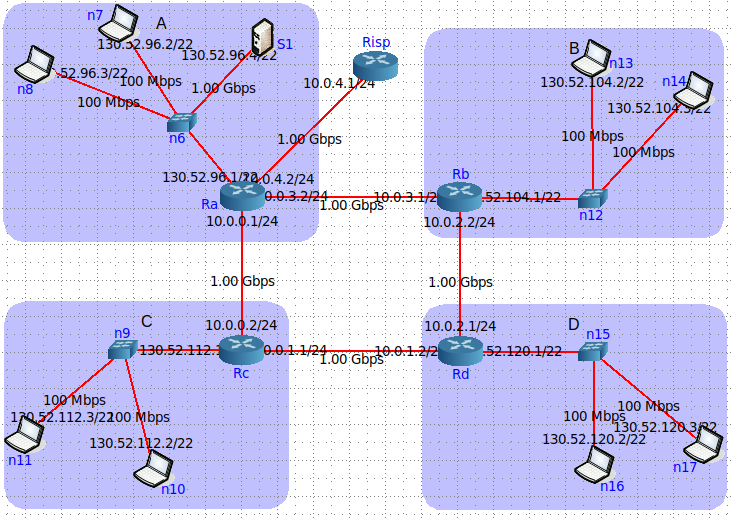
\includegraphics[width=0.5\textwidth]{images/parte3/core2.png}
    \caption{Topologia CORE com IPs atribuídos manualmente}
\end{figure}

\begin{figure}[!htb]
    \centering
    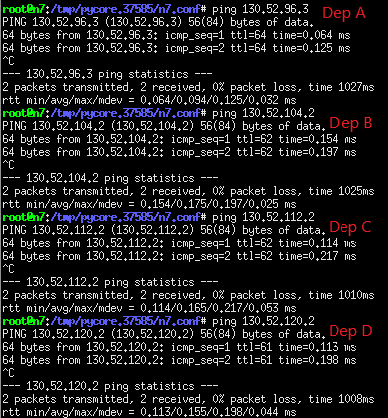
\includegraphics[width=0.5\textwidth]{images/parte3/pings_final.png}
    \caption{Ping de um laptop do Dep A (n7) para um laptop de cada departamento}
\end{figure}

\clearpage
\section{Conclusão}

Na primeira parte do trabalho, foi feita uma análise ao protocolo IPv4. Para tal, realizamos uma topologia CORE e analisamos o tráfego ICMP referente. Para além disso, estudamos o caso particular da fragmentação de pacotes IPv4. Nesta parte do trabalho, consolidamos os nossos conhecimentos sobre a transmissão de pacotes entre vários equipamentos ligados a uma rede, em específico, usando o protocolo IPv4.

Na segunda parte, construímos outra topologia CORE, com 4 departamentos distintos, de forma a estudar o comportamento destes entre si, nomeadamente das rotas que os pacotes seguem. Vimos ainda como poderíamos manipular endereços IP, podendo assim criar sub-redes personalizadas. Nesta parte, percebemos melhor como funcionam as interações entre sub-redes e aprendemos a manipular as rotas entre estas. Deparamo-nos, ainda, com a dificuldade de atribuir endereços IP manualmente a equipamentos de sub-redes.

\end{document}